\documentclass{beamer}

% Theme choice (you can change to Madrid, CambridgeUS, etc.)
\usetheme{Madrid}

% Optional packages
\usepackage[utf8]{inputenc}
\usepackage{graphicx} % for including images
\usepackage{amsmath, amssymb} % for math symbols
\usepackage{hyperref} % for clickable links
\usepackage{tikz}

% Title info
\title[Short Title]{Factor Models of Returns}
\author[Your Name]{Oden Petersen}
\date{\today}

% Section headers
\AtBeginSection[]{
	\begin{frame}
	\vfill
	\centering
	\begin{beamercolorbox}[sep=8pt,center,shadow=True,rounded=True]{title}
		\usebeamerfont{title}\insertsectionhead\par%
	\end{beamercolorbox}
	\vfill
	\end{frame}
}

\begin{document}

% Title page
\begin{frame}
	\titlepage
\end{frame}

\begin{frame}{About Me}
\end{frame}

% Table of contents
\begin{frame}{Outline}
	\tableofcontents
	%% Good to include concrete data examples throughout
\end{frame}

% Section 1
\section{Securities Markets}

\begin{frame}{Spot Transactions}
	If I give you $q$ units of some asset $A$, and you give me $\$p$, then:
	\begin{itemize}
		\item I have \textbf{sold} $q$ units of $A$ to you at $\frac{\$p}{q}$
		\item You have \textbf{bought} $q$ units of $A$ from me for $\frac{\$p}{q}$
	\end{itemize}

	Buying and selling are collectively called `trading'.

	% Stock image of retail store
\end{frame}

\begin{frame}{Securities Markets and Exchanges}
	The \textbf{\textcolor{blue}{market}} is whatever lets you make trades. When we don't care who we trade with, we can just `trade with the market'.

	A \textbf{\textcolor{red}{securities} \textcolor{blue}{market}} for some asset $A$, open at a time $t$, is any \textcolor{red}{standardised} \textcolor{blue}{way for traders to reach agreements to buy or sell} $A$ at a specified \textbf{settlement time} $T\geq t$.

	\pause

	For example, $T=\ldots$
	\begin{itemize}
		\item $t$ (`spot', e.g. blockchain)
		\item $t+1, t+2, \ldots$ (`clearing', e.g. equities)
		\item Last Thursday of month (`futures')
	\end{itemize}

	\pause
	If you agree to give something to someone, you have an \textbf{obligation}. If someone agrees to give you something, you have a \textbf{right}.

	\begin{block}{Counterparty Risk}
		If I have an agreement with $P_1$ to buy $10$ units for $\$p_1$ at $T$, and an agreement with $P_2$ to sell $10$ units at $\$p_2$ at $T$, and no further rights/obligations, am I guaranteed to meet my obligations?
	\end{block}
\end{frame}

\begin{frame}{Settlement and Clearing}
	A \textbf{securities exchange} is a centralised venue serving a securities market for \textbf{exchange participants} (e.g. ASX, NYSE, TSE, HKEX, LME).

	\begin{columns}[t]
		\begin{column}{0.48\textwidth}
			\begin{center}
				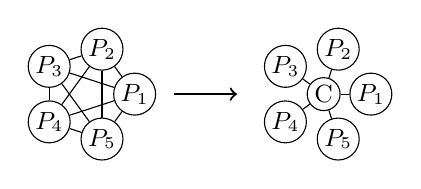
\begin{tikzpicture}[baseline, every node/.style={circle, draw, fill=white, inner sep=1pt, font=\small, minimum size=2mm}]
					\foreach \i in {1,...,5} {
						\node (n\i) at ({72*(\i-1)}:0.6) {$P_{\i}$};
					}
					\foreach \i in {1,...,5} {
						\foreach \j in {1,...,5} {
							\ifnum\i<\j
								\draw (n\i) -- (n\j);
							\fi
						}
					}

					\draw[->, thick] (1.1,0) -- (1.9,0);

					\begin{scope}[xshift=3cm]
						\node (c) at (0,0) {C};
						\foreach \i in {1,...,5} {
							\node (n\i) at ({72*(\i-1)}:0.6) {$P_{\i}$};
							\draw (c) -- (n\i);
						}
					\end{scope}
				\end{tikzpicture}
			\end{center}
			\pause
			\begin{block}{Netting}
				Centralisation allows for \textbf{netting} of rights and obligations. For any settlement time $T$, I only need to keep track of the difference between money owed to and by me, and units owed to and by me.
			\end{block}
		\end{column}

		\pause
		\begin{column}{0.48\textwidth}
			\begin{block}{Collateralisation}
				At certain intermediate times $t'$ ($t\leq t'\leq T$), participants may be required to physically give (`post') something to the exchange to \textbf{collateralise} their obligations.
				\begin{enumerate}
					\item Money (`margin') %Explain the term "futures type settlement" and "stock type settlement"
					\item Assets (`locate'/`borrow') %"Borrow" is only if you don't own the thing
				\end{enumerate}
				If an agreement made on the exchange gives you rights to money or assets, this is typically as good as posting actual money or assets.
			\end{block}
		\end{column}
	\end{columns}
\end{frame}

\begin{frame}{Summary}
	\begin{enumerate}
		\item \textbf{Trading} is swapping money and assets
		\item A \textbf{market} is whatever you use to trade
		\item A \textbf{securities market} is a standardised way to agree to trades
		\item Agreements consist of \textbf{rights} and \textbf{obligations}
		\item A \textbf{securities exchange} is a centralised trading venue
		\item After trades are agreed to, they will be \textbf{settled} in some standardised way
		\item Traders may be obligated to post assets ('locate') or money ('margin')
	\end{enumerate}
\end{frame}

\section{Trading}
\begin{frame}{Trade Formation}
	% Order books
	% aggressive vs passive (taking/making)
	% Latency
\end{frame}

\begin{frame}{Market Data \& Market Prices}
	% Theoretical value
	% Price chart. Various position charts.
\end{frame}

\begin{frame}{Valuation}
	%Mark to market valuation
	%Portfolio value
	\begin{block}{Portfolio Capitalisation}
		Because of collateralisation requirements, \textbf{the amount you can trade (and therefore your potential profits) are constrained by how much money you have at the exchange.}
	\end{block}
	
	% Portfolio value integration by parts: pos dprice ~ price dpos
	% Dot products explainer
	% Portfolio returns and log-returns
\end{frame}

\begin{frame}{Transaction Costs}
	% Fees
	% Spreads
	% Persistent price impact

	% Augmented P&L integral

	% Market impact
		% Adverse selection
		% Trade volumes and liquidity reinforce each other
\end{frame}

\begin{frame}{Uncertainty}
	%Dutch books & FTAP & Q vs P quant
	%(No-)Arbitrage (buy low sell high. Setup for statarb later)
\end{frame}

\begin{frame}{Decision-Making}
	%Systematic, semi-systematic, discretionary
	%High-touch, low-touch
	% What is point of systematic? (consistency, breadth)
		% “We’re mediocre traders, but our system never has rows with its girlfriends — that’s the kind of thing that causes patterns in markets.” Nick Patterson RenTech
\end{frame}

\section{Portfolio Management}
\begin{frame}{Risk}
	% Trading is zero-sum. So why do we do it
	% Risk = variance
		% "Cars have brakes so you can drive faster." Ben Rady
	% Portfolio variance and covariance
\end{frame}

\begin{frame}{Decision Theory}
	%Markowitz frontier
	%Pareto optimality
	%Security market line
	%Markowitz solution
		%Estimation difficulties
	%VNM & kelly theory
\end{frame}

\begin{frame}{Capital Asset Pricing Model}
	% Arbitrage arguments
	%Efficient Markets
	%Index investing. (Stats?)
		%Why ASX200 and not all ords (microstructure)
		%Grossman-Stiglitz Paradox
\end{frame}

\begin{frame}{Factor Models}
	% Mathematics
	% Sectors
	% Fama French
	% Factor models approximate cov matrix
		% Why cov matrix approximation is hard to begin with - paleologo 4.5.2 faq 4.5
	% Overrepresentation -> equal weighting (equal weighting index)
	% Factor loadings can't be centred (paleologo 4.4.1) unless an "equal weighting" vector is included
	% Types (paleologo 4.6):
		% characteristic
		% statistical
			% Latent factors (eg principal components)
		% macroeconomic
			% Fama macbeth
\end{frame}

\begin{frame}{Statistical Arbitrage}
	% Factor model stat arb (eg pairs trading), kalman filter with factor cov structure
\end{frame}

\section{Options Trading}
	%If black scholes was true options markets wouldnt exist

	% Linear regression mathematics
		% Matrix multiplication
	% Regularisation
	% Factor models in options pricing
		% Diagnosing issues with the model eg because black scholes is wrong ("all models are wrong")
\end{document}
